\documentclass[12pt, twoside]{article}
\usepackage[letterpaper, margin=1in, headsep=0.5in]{geometry}
\usepackage[english]{babel}
\usepackage[utf8]{inputenc}
\usepackage{amsmath}
\usepackage{amsfonts}
\usepackage{amssymb}
\usepackage{tikz}
\usetikzlibrary{quotes, angles}

\usepackage{pgfplots}
\pgfplotsset{width=9cm,compat=1.9}
\usepgfplotslibrary{statistics}
\usepackage{pgfplotstable}

\usepackage{venndiagram}

\usepackage{graphicx}
\usepackage{enumitem}
\usepackage{multicol}
\usepackage{hyperref}

\newif\ifmeta
\metatrue %print standards and topics tags

\title{IB Mathematics}
\author{Chris Huson}
\date{November 2021}

\usepackage{fancyhdr}
\pagestyle{fancy}
\fancyhf{}
\renewcommand{\headrulewidth}{0pt} % disable the underline of the header
\raggedbottom


\fancyhead[LE]{\thepage}
\fancyhead[RO]{\thepage \\ Name: \hspace{4cm} \,\\}
\fancyhead[LO]{BECA / IB Math 02-Descriptive Statistics\\* 19 November 2021}

\begin{document}

\subsubsection*{2.3 Quiz: Box and whisker plots}
\begin{enumerate}
\item Determine whether each set of data is quantitative or categorical, and discrete or continuous by circling the appropriate labels.
  \begin{enumerate}[itemsep=0.5cm]
    \item The favorite ice cream flavors of 20 people\\. \hfill quantitative categorical; discrete continuous
    \item The genres of 20 top movies \hfill quantitative categorical; discrete continuous
    \item The number of kittens in each of 50 litters\\. \hfill quantitative categorical; discrete continuous
    \item The number of empty beds in a hospital during flu season\\. \hfill quantitative categorical; discrete continuous
    \item The number of students in the 9th, 10th, and 11th grades\\.  \hfill quantitative categorical; discrete continuous
    \item The weight of each bag of skittles\\. \hfill quantitative categorical; discrete continuous
  \end{enumerate} \vspace{0.5cm}

\item Find the 5-figure summary statistics of the following data:
  \begin{center}
  15 4 13 6 15 12 9 7 3
  \end{center}
  \begin{enumerate}[itemsep=0.7cm]
    \item Rewrite the data in order.
    \item Minimum =
    \item 1st Quartile =
    \item Median =
    \item 3rd Quartile =
    \item Maximum =
    \item Range =
    \item IQR =
  \end{enumerate} \vspace{0.5cm}

\newpage
\item The box-and-whisker plot represents the examination scores of a group of students.
  \begin{center}
  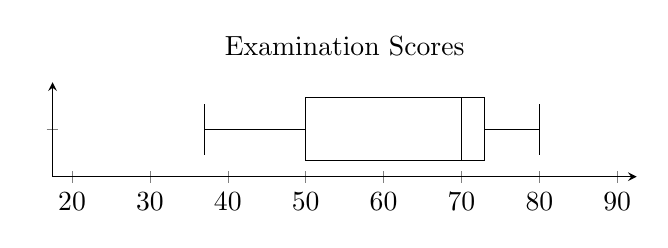
\begin{tikzpicture}[scale=1.0]
    \begin{axis}[
        title={Examination Scores},
        axis lines=left,
        xmin=30, xmax=80,
        y=1cm,
        ytick={1},
        yticklabels={},
      enlargelimits=0.25,
        ]
        %\addplot+ [boxplot]
        %table {3-11_IB-exam.txt};
       \addplot [boxplot prepared={draw position=1,
            lower whisker=37, lower quartile=50,
            median=70,
            upper quartile=73, upper whisker=80,
            %average=28,
            },
        ] coordinates {};
    \end{axis}
    \end{tikzpicture}
  \end{center}
  \begin{enumerate}
    \item Write down each value:
    \begin{enumerate}
      \begin{multicols}{3}
        \item median =
        \item $Q_1 = $
        \item max =
      \end{multicols}
    \end{enumerate} \vspace{0.5cm}
    The range of the scores is 43 marks, and the interquartile range is 23 marks. \vspace{0.5cm}
    \item Find the value of
    \begin{enumerate}
      \item the minimum score; \vspace{1cm}
      \item the third quartile. 
    \end{enumerate}
  \end{enumerate}

\item Draw a box and whiskers plot of the five-figure summary on the grid. Use a ruler for full credit. \vspace{0.25cm}\\
min = 3, $Q_1=6$, median = 10, $Q_3=13$, maximum = 16

\begin{center}
  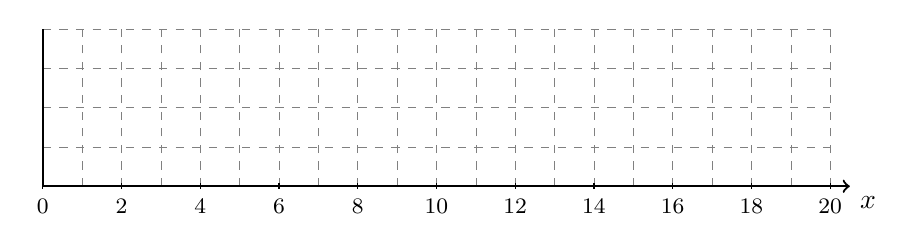
\begin{tikzpicture}[scale=.5]
    \draw [help lines, dashed] (0,0) grid (20,4);
    \draw [thick, ->] (0,0) -- (20.5,0) node [below right] {$x$};
    \foreach \x in {0,2,4,6,8,10, 12, 14, 16, 18, 20}
      \draw[shift={(\x,0)},color=black] (0pt,2pt) -- (0pt,-2pt) node[below] {\footnotesize $\x$};
    \draw [thick, -] (0,0)--(0,4);
  \end{tikzpicture}
\end{center}

\item Find the mean of the following set of numbers (show the substitution of the values into the formula for full credit):
  \begin{center}
    109, 110, 114, 115, 117
  \end{center}

\newpage
\item Given the following set of 15 data:
    \begin{center}
    2, 4, 4, 5, 5, 6, 8, 9, 11, 11, 15, 15, 15, 16, 19
  \end{center}
  \begin{enumerate}
    \item Write down the mode \vspace{1cm}
    \item Find the median. \vspace{1.5cm}
    \item Find the interquartile range. \vspace{1cm}
    \item Draw a box and whiskers plot of the data on the axis below. \vspace{1cm}
      \begin{center}
        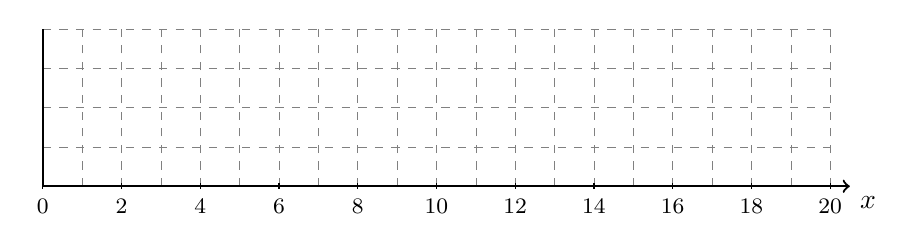
\begin{tikzpicture}[scale=.5]
          \draw [help lines, dashed] (0,0) grid (20,4);
          \draw [thick, ->] (0,0) -- (20.5,0) node [below right] {$x$};
          \foreach \x in {0,2,4,6,8,10, 12, 14, 16, 18, 20}
            \draw[shift={(\x,0)},color=black] (0pt,2pt) -- (0pt,-2pt) node[below] {\footnotesize $\x$};
          \draw [thick, -] (0,0)--(0,4);
        \end{tikzpicture}
      \end{center} \vspace{0.2cm}
      \item Find the mean.
    \end{enumerate} \vspace{1cm}

\item Given the linear function $f(x)=-\frac{2}{3}x+4$.
\begin{multicols}{2}
\begin{enumerate}
  \item Write down it's slope.\\ $m=$
  \vspace{0.25cm}
  \item Write down it's $y$-intercept.\\ $b=$
  \vspace{0.25cm}
  \item Draw the function $f$ on the grid.
  \vspace{1cm}
  \item Label the $x$-intercept with its coordinates as an ordered pair.
\end{enumerate} \vspace{.5cm}
  \begin{center} 
  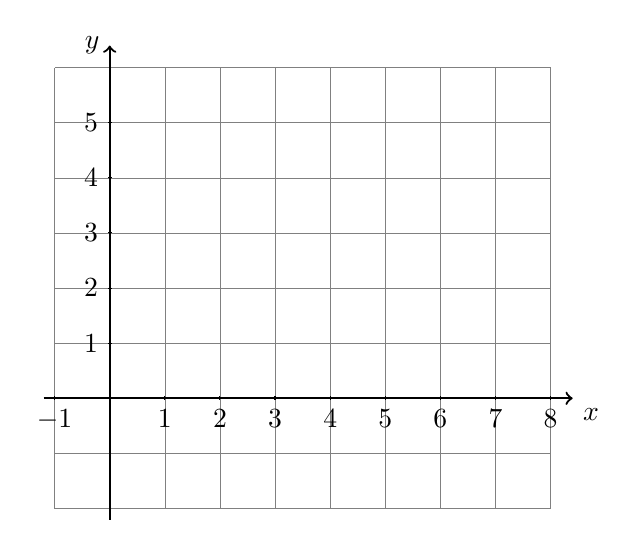
\begin{tikzpicture}[scale=0.7]
    \draw [help lines] (-1,-2) grid (8,6);
    \draw [thick, ->] (-1.2,0) -- (8.4,0) node [below right] {$x$};
    \draw [thick, ->] (0,-2.2)--(0,6.4) node [left] {$y$};
    \foreach \x in {-1,1,2,...,8} \draw (\x cm,1pt) -- (\x cm,-1pt) node[anchor=north] {$\x$};
    \foreach \y in {1, 2, 3, 4, 5} \draw (1pt,\y cm) -- (-1pt,\y cm) node[anchor=east] {$\y$};
    %\draw [thick, <->,smooth,samples=20,domain=-2.25:4.5] plot(\x,0.667*\x+2);
    %\fill (3,4) circle[radius=0.1] node[below right]{$Q$};
  \end{tikzpicture}
  \end{center}
\end{multicols}

\newpage
\item The weight of a pumpkin $w$ in pounds over a period of time $t$ measured in weeks is shown in the table.
\begin{enumerate}
  \item Plot the data as points on the grid.
  \item Draw a line of best fit on the graph.
\end{enumerate}
  \begin{center} 
  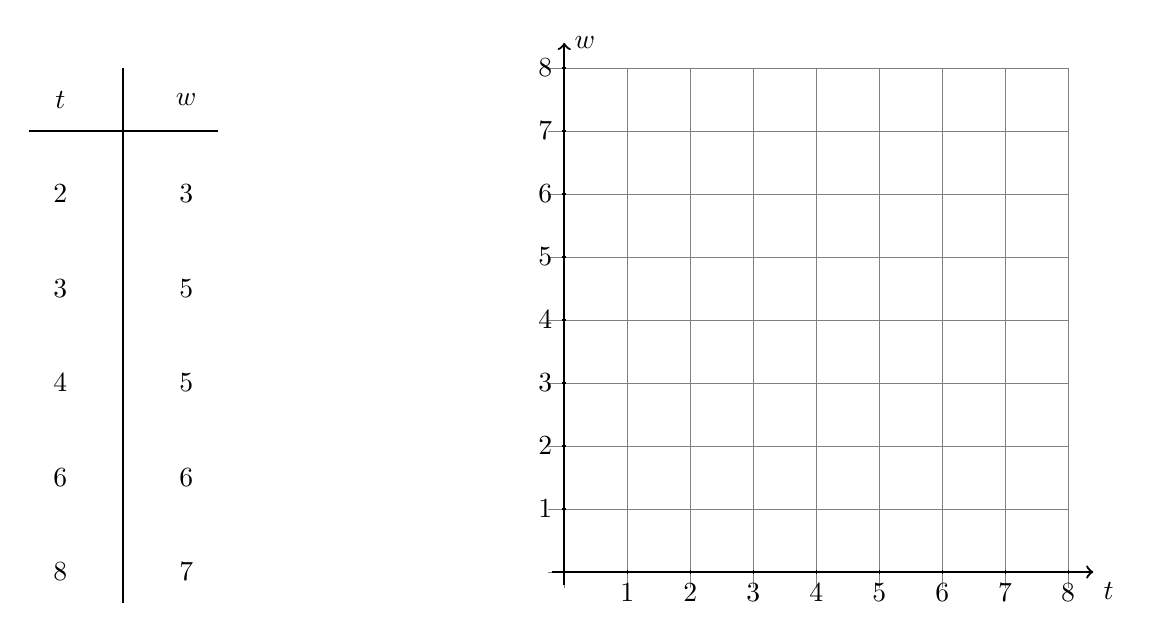
\begin{tikzpicture}[scale=0.8]
    \draw [help lines] (-0.25,-0.25) grid (8,8);
    \draw [thick, ->] (-0.2,0) -- (8.4,0) node [below right] {$t$};
    \draw [thick, ->] (0,-0.2)--(0,8.4) node [right] {$w$};
    \foreach \x in {1,2,...,8} \draw (\x cm,1pt) -- (\x cm,-1pt) node[anchor=north] {$\x$};
    \foreach \y in {1,2,...,8} \draw (1pt,\y cm) -- (-1pt,\y cm) node[anchor=east] {$\y$};

    \draw [thick] (-7,-0.5) -- (-7,8);
    \draw [thick] (-8.5,7) -- (-5.5,7);
    \node at (-8,7.5){$t$}; \node at (-6,7.5){$w$};
    \node at (-8,6){$2$}; \node at (-6,6){$3$};
    \node at (-8,4.5){$3$}; \node at (-6,4.5){$5$};
    \node at (-8,3){$4$}; \node at (-6,3){$5$};
    \node at (-8,1.5){$6$}; \node at (-6,1.5){$6$};
    \node at (-8,0){$8$}; \node at (-6,0){$7$};
  \end{tikzpicture}
  \end{center}

  \subsubsection*{Arithmetic sequences}
Terms: $u_n=u_1 + d(n-1)$\\[0.25cm]
Sum: $\displaystyle S_n= \frac{n}{2}(u_1 + u_n)$\\
  
\item Given the arithmetic sequence $11,17,23,29, \dots$
  \begin{enumerate}[itemsep=1cm]
    \item Find the common difference $d$.
    \item Write down the next term, $u_5$.
    \item Find the tenth term.\vspace{0.75cm}
    \item Find the sum of the first ten terms.
  \end{enumerate} \vspace{2cm}

  

\end{enumerate}
\end{document}